\documentclass{sig-alternate}
\usepackage{mdwlist}
\usepackage{url}
\usepackage{graphicx}

\begin{document} 

\title{Automatic Harmonization}
\subtitle{Viewed as a Machine Translation Problem}
\numberofauthors{2}
\author{
\alignauthor Nicole Limtiaco \\ \email{limni@seas.upenn.edu} \\ Univ. of Pennsylvania \\ Philadelphia, PA
\alignauthor Rigel Swavely \\ \email{rigel@seas.upenn.edu} \\ Univ. of Pennsylvania \\ Philadelphia, PA}
\date{}
\maketitle

\begin{abstract}
  \textit{In the past, approaches to automatic harmonization of a melody
  have taken two forms: using rules provided by music theory or by predicting
  the chord under the melody. This attempt approaches the problem from a machine translation perspective, 
  modeling the melody of a song as the source language and each harmony as a target language.
  By generating the harmony lines explicitly rather that generating them as a
  consequence of the chord on each beat, we hope that the algorithm will be able to create
  more cohesive, creative works.}

  \textit{In order to accomplish this, we use a translation model to represent the probability
  of one note harmonizing with another note. Additionally, we use a language model to represent
  a note following a phrase of notes in the same line of music. A perplexity metric is used to 
  evaluate the generated models. If there is time, we hope to incorporate human evaluation
  and data driven rhythmic variation.}
\end{abstract}

\section{Introduction}
\label{sec:intro}
Many would consider music composition to be an art form that is accomplished
primarily through human creativity. Writing music is a process that seems to require
complex thought which fundamentally cannot be boiled down to a list of straightforward
processes. Our project aims to answer the question, ``Can computers imitate the complex
and creative process of composing music?'' We narrow the question down to the more specific
and well-defined problem of generating a group of harmony lines for a given melody line.

We will define a \textit{melody} as a sequence of input \textit{notes}, where each note contains information
about pitch and timing. A \textit{harmony} will be a sequence of output notes which are produced with
the constraint that the sequence of notes supports the input melody. We define the term \textit{voice}
to be some sequence of notes, either a melody or one of the harmonies, with a certain set of identifying 
characteristics. For example, the bass part in rock music is one type of voice and the soprano's part in an 
opera is another. The end result we wish to generate will be a group of $n$ voices---the input melody and 
$n-1$ automatically-composed harmonies---that, when played together, sound coherent and pleasant.

We propose to approach the problem from the view point of machine translation, where the input language
is the melody and the target languages are the specific harmony voices to be generated.

\section{Related Work}
\label{sec:related_work}
Automatic harmonization is a subset of the automatic musical composition problem,
which dates as far back as the field of artificial intelligence itself. Perhaps
the earliest work in automatic composition is Hiller and Isaacson's
\textit{Illiac Suite} \cite{hiller1959experimental}, which is widely accepted as being the first
musical piece composed by an electronic computer. Hiller and Isaacson
used a generate-and-test method that generated musical phrases psuedo-randomly and 
kept only those that adhered to a set of music-theory-inspired heuristics. 

Staying in line with the use of musical rules, Ebcio\v{g}lu \cite{Ebci̇oğlu1990145} provided a break-through 
in the specific field of automatic harmonization through his CHORAL system. CHORAL, 
bolstered by about 350 music-theory and style rules expressed in first order logic, performed the task of
writing four-part harmonies in the style of J.S. Bach. With these logical predicates, Ebcio\v{g}lu 
reduced the problem of composing a harmony to a simple constraint satisfaction problem. Similar 
later works, notably by Tsang \& Aitkin \cite{tsang1991}, also crafted the harmonization problem as a 
problem in constraint satisfaction, but with a significantly smaller amount ($\sim$20) of musical rules.
The result of these constraint-based works were musically sensible; however,
crafting the constraints such that the output is musical requires deep, human knowledge about music in general and about the style of music to be produced in particular.

More recent works have put data-driven methods into use in order to infer the patterns that govern real compositions. A simple case-based model implemented by Sabater \textit{et al.} \cite{Sabater98usingrules} was built to generate
accompanying chords for a melody line. To a choose a harmony chord for a given context of previous
harmony chords and the currently sounding melody note, the system would check a case base to see if any
cases had the same harmony context and melody note and use the corresponding harmony chord if such a 
match were found. Musical heuristics were used to generate a chord if no match was found in the case base.
An automatic harmonizer utilizing neural networks was also built by Hild \textit{et al.} \cite{NIPS1991_576}  to produce a harmony
chord for a given melody quarter beat. Input features to the network included harmony context, current melody pitch,
and whether or not the beat was stressed.

As these examples show, the previous harmony context and the melody pitch are important signals in deciding
what the current harmony phrase should be. Many works have been conducted that model these signals using
n-gram Markov Models. A Markov model assigns probabilities to some event $C_{t}$ conditioned on a limited history
of previous events [$C_{t-1}\ldots\\
C_{t-n}$], implictly making the assumption that the event $C_{t}$ depends only on a 
small amount of information about its context. For example, a system called MySong produced by Simon \textit{et al.} \cite{export:64277}
generates chord accompaniment given a vocalized melody by using a 2-gram Markov model for the harmony
context and a 2-gram Markov model for the melody context. A similar system implented by Scholz \textit{et al.} \cite{4959518},
which also generates chord accompanimants, experimented with 3-gram to 5-gram Markov models and incorporated
smoothing techniques commonly seen in NLP to account for cases in which the model has not seen a context
that is present in the test data. Most recently, Raczy\'{n}ski \textit{et al.} \cite{doi:10.1080/09298215.2013.822000} uses discriminative Markov models that
model harmony context, melody context, and additionaly the harmony relationship to the tonality.

A recent senior design project out of the University of Pennsylvania by Cerny \textit{et al.} \cite{UAMP} also used melody pitch and previous harmony context
as their main signals for determining the next harmony chord to generate. However, they used these
signals as inputs to an SVM classifier, as opposed to training a Markov model. 

We propose to solve the problem differently from the previous works by predicting the individual harmony lines that make up
a multi-part arrangement, as opposed to predicting full chords to play under the given melody. We would like to use machine
translation techniques to accomplish this task, but our problem differs in an interesting way from standard machine translation
applications in that we are translating from one language (melody voice) to many languages ($n - 1$ harmony voices) instead of one language to one other language. Looked at from a different perspective, we can view our problem as a sequence of translations from many source languages to one target language. The sources are the melody voice and all the harmony voices, if any, that have been produced so far; the target is the harmony voice we would like to produce next. Though limited work has been done on the multi-source translation problem, Och and Ney \cite{franzjosefochhermannney2001} produced a work describing several ways of altering standard methods to solve the problem.

\section{System Model}
\label{sec:sys_model}
\subsection{Motivating the Machine Translation Approach}

The previous data driven approaches applied to automatic harmonization all share in the fact that they predict the chords to be played under the input melody. We believe automatic harmonization via chord prediction imposes two major limitiations: a limited set of produceable chords and a lack of interesting movement within the individual parts. 

In the best case, chord prediction will alow only the generation of those chords seen in the training data. In more restrictive set-ups where classification algorithms are used, the chord predicted is based on a classifier choosing from a relatively small number of chord classes. Some chord prediction systems do not generate individual parts at all, but rather view the harmony output as just the underlying chord sequence generated. If individual parts are produced, the notes for each part are chosen from the predicted chord, not based on the context of previous notes in that part. Chord prediction further forbids any interesting rhythmic variation because all the notes in the harmony are played at the same time. This is a far cry from actual musical arrangements, whose parts can move independently of each other and at times produce non-conventional chords. In fact, this approach differs greatly from how actual composers create multi-part arrangements, creating musical phrases in each part rather than purely choosing chords to sound on each beat.

Instead of chord prediction, we propose predicting the sequence of notes in the individual parts in such a way that will allow them to sound coherent when played all at once. A model like this will allow unseen chords to be produced because there is no restriction on which groups of notes can sound together, only on which notes can be produced. Although, we would of course hope that our system only generates groups of notes that sound pleasant together in context. Furthermore, the system can be made to encourage interesting movement within the individual parts, for example by taking the part's context into account or by allowing rhythmic variation. In order to produce interesting voices individually while still managing to have them sound coherent when played together, we turn to machine translation techniques.

Modeled as a machine translation problem, the problem of automatic harmonization has the given melody voice as a source language 
and the desired harmony voices as the target languages. Though we can map these two problems' inputs and outputs cleanly, we
need to build more intuition as to why a machine translation approach makes sense. There are two main analogies between natural language and musical voices that lead us to believe that machine translation techniques could successfully solve the problem of automatic harmonization. The first analogy is that both natural languages and musical voices have a sense of ``word translations''. Just as there may be several words in the target language that could be sensible translations of a given word in the source 
langauge, there are also several notes in the harmony voice that can harmonize well with an input melody note. Importantly, 
however, it is not the case that any note can harmonize well with the melody note. Some notes will sound dissonant when played together and still other notes may not be in the harmony language at all, since harmony voices can have specified note
ranges. 

The second analogy that allows us to view this problem as a machine translation problem is that, like 
natural language, only certain strings of tokens (i.e. notes) are sensible in a given harmony voice. For example,
the statement ``colorless green ideas sleep furiously'' contains all english words but is unlikely to
be understood by an english speaker because the string of words in not sensible based on the rules of our
language. Similarly, a random sequence of notes may not sound sensible in the context of its
harmony voice, if the notes are even recognized as music at all. This analogy shows us that it should be
possible to generate new content in the harmony voice similar to how machine translation algorithms are 
able to generate new natural language content.

\subsection{System Design Overview}

In line with the analogies explained above, we will solve the automatic harmonization problem using two probabilistic models commonly employed by statistical machine translation: the translation model and the language model. The translation model will provide the probability, $P_{TM}(M | H)$, of a melody line sounding with a given a harmony line, and the language model will provide the probability, $P_{LM}(H)$, of some harmony line being generated. Specifically, the translation and language models will be given by: \\

$p_{TM}(M | H) = \Pi_{i = 1}^{l} P[m_{i} | h_{i}]$\\

$p_{LM}(H) = \Pi_{i = 1}^{l} P[h_{i} | h_{i - 1} \ldots h_{i - n}]$\\

The description of the language model is just that of a Markov Model with n-gram size $n$. The details of the Markov Model will be described in the implementation section, but for now suffice it to say that we will assume the probability of seeing some harmony note $h_{i}$ is based only on the identities of the previous $n$ harmony notes. 

Combining the probabilities given by the two models, we can determine $P(H | M)$, the probability of some harmony line given a melody line. By Baye's rule we have that: \\

$P(H | M) = \frac{P(M | H)P(H)}{P(M)}$\\

Given a melody line $M$, the goal is to find some harmony line $H$ that maximizes the probability $P(H | M)$. More formally we want to find $H$ where\\

$H = argmax_{H}p(H | M) = p_{TM}(M | H)p_{LM}(H)$.\\

A training algorithm will be used to produce the tranlsation and language models from music data. There will also be a decoder
algorithm which will use the language and tranlation models to determine the best harmony line given a melody line. Below is a graphical overview of the model just described.\\

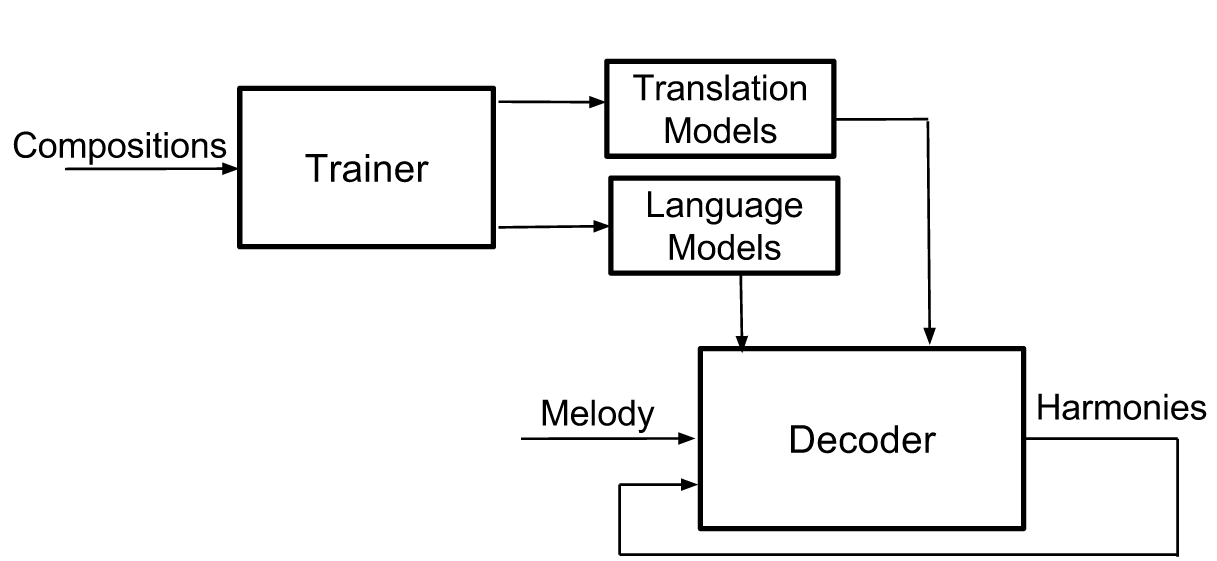
\includegraphics[scale=0.2]{design_overview.png}\\

Up until this point, we have only explained the model in terms of translating from the melody into one harmony voice. However, the goal is to produce $n - 1$ harmony parts for the given melody in order to produce a complete $n$-part arrangement. In order to do this, we view the decoding portion of the system as a sequence of multi-source translations where the source languages are the melody voice and all of the harmony voices generated so far. The generated harmony voice will maximize the product of the probability given by its language model and the probabilities given by all the relevant translation models, where there is an individual translation model from each source voice to the voice being generated. More formally, given a set $S$ of source voices, the multi-source version of translation attempts to find a harmony line $H$ such that\\

$H = argmax_{H}p(H | M) = (\Pi_{S}\ p_{TM}(S | H)) \cdot p_{LM}(H)$.\\

Viewing translation as a sequence of generation steps then introduces the problem of determining the best order for the parts to be generated. Since each part is constrained by the parts generated previously, one would expect that the order in which the parts are generated will have an observable affect on the output. Indeed, our experiments have shown that the quality of the output varies greatly among different generation orderings. Details about how we plan to choose an optimal ordering will be discussed in the implementation section.

\section{System Implementation}
\label{sec:sys_implement}
\subsection{Programming Language}
Since we anticipated that the development of the system would involve a significant amount of experimentation, we decided to implement it in Python because of the language's ease of development and large amount of library resources, especially in the realm of machine translation and general NLP. Python's concise syntax, even when dealing with complex data structures, allowed us to focus on developing the core of our system.

\subsection{Data Collection and Interaction}
In order to train the language and translation models, we needed a large corpus of music data and a way to interact with it. For this,
we used third-party software called Music21 \cite{Cuthbert_music21:a}, a library developed at MIT which provides a simple interface for querying the library's database of musical scores. Music21 parses MusicXML, a type of encoding for standard music notation, into Stream objects which can then be queried for any of the information contained in the notation including key, tempo, and notes with pitch and timing. Additionally, the Music21 package has over $2,000$ compositions, mostly written by classical composers. We have primarily trained on the package's Bach chorales, of which there are $402$.

\subsection{Note Representation}
We represent notes in the language and translation models as strings of pitch class and octave number, collectively defining the note's pitch. For example, the representation of middle C would be ``C4''. Timing properties are currently not stored in the note representation because we have not yet integrated timing variation into the system. If timing were to be integrated, we propose adding an additional number to the end of the note's string representation describing the note's quarter length. For example, a whole note would have the number $4$ added to it's representation and an eighth note would have the number $0.5$ added to its representation. 

We also consider rests, moments of silence in the composition, to be ``notes'' in our model. They are represented by the string ``R''. Including rests makes it possible to harmonize a melody note with silence, thus offering some opportunity for rhythmic variation. However, including rests does pose the potential problem of producing too much silence, which is not optimal for music generation software. For example, imagine we are using a language model of n-gram size $2$, if $P(R | R)$ and $P (R | R\ R)$ are both relatively high, once we produce one rest, we may very well produce rests for the remainder of the song. Therefore, for fear of continually producing rests, we treat all contiguous sequences of rest symbols in a composition as one rest ``R'' in the model.

Measure bars are also modeled as ``notes'' in our system. They are represented by the string ``BAR''. A special measure bar, the bar at the end of last measure in the song, is given a special representation: ``END''. These notes are slightly different in that they are only present in our language model. ``BAR'' and ``END'' can only be harmonized with actual measure bars and song end in the given melody line, so there is no need to include them in the translation model. The motivation for including ``BAR'' and ``END'' in the language model is that they provide information about where in the composition the system is trying to produce notes. This information is helpful because some notes may be more likely to start or end measures and some sequences of notes may be more likely to end a song. Coming back to the analogies between languages and musical voices, the ``BAR'' and ``END'' symbols can be likened to punctuation marks, which can give very strong cues about which words to generate, given that a string of natural language, a sentence for example, is about to end.

\subsection{Model Generation}
The translation and language models are implemented as nested dictionaries. The outer dictionary maps the given parameter, $A$, to the inner dictionary, which maps the unknown parameter, $B$, to the probability $P(B | A)$. In the case of the translation model, $A$ is a harmony note and $B$ is a melody note, while in the language model, $A$ is the sequence of $(i - 1) ... (i - n)$ harmony notes and $B$ is the $i^{th}$ harmony note.

The probabilities are calculated based on the counts of the events in the training compositions, plus smoothing techniques applied so that no event is assigned a zero probability. For now, we omit the smoothing techniques for the ease of explanation. Formally, the translation probabilities are given by:\\

$P(m_{i} | h_{j}) = \frac{count(m_{i} \wedge h_{j})}{count(h_{j})}$\\

and the language ngram probabilities are given by: \\

$P(h_{i} | h_{i - 1} ... h_{i - n}) = \frac{count(h_{i} \wedge h_{i - 1} \wedge ... \wedge h_{i - n})}{count(h_{i - 1} \wedge ... \wedge h_{i - n})}$\\

The event $m_{i} \wedge h_{j}$, as seen in the translation probability formula, occurs whenever the note $m_{i}$ is sounding in the melody at the same time as $h_{j}$ is sounding in the harmony. Since we currently only model the notes as pitches, we consider two notes to be harmonizing with each other as long as their pitches play concurrently, regardless of when either note begins or ends or how long it lasts. To compute these counts, we iterate through each note $m_{i}$ in the melody and update the counts for event $m_{i} \wedge h_{j}$ for all notes $h_{j}$ that have any portion of their duration sounding at the same time as any portion of the duration of $m_{i}$.

The event $h_{i} \wedge ... \wedge h_{i - n}$, as seen in the ngram probability formula, occurs whenever the notes $h_{i - n}, h_{i - n + 1}, ..., h_{i}$ appear contiguously in that order in the haromny line. 

In the language model, to avoid any events having zero probability, we use LaPlace smoothing, also known as additive smoothing. Specifically, for some smoothing constant $\alpha$, the language ngram probabilities are given by: \\

$P(h_{i} | h_{i - 1} ... h_{i - n}) = \frac{count(h_{i} \wedge h_{i - 1} \wedge ... \wedge h_{i - n}) + \alpha}{count(h_{i - 1} \wedge ... \wedge h_{i - n}) + (48\alpha)}$\\

The constant $48$ in the equation above is meant to be the number of possible note values for the variable $h_{i}$. It is derived from the fact that there are 12 notes in each octave and that 4 is a very liberal estimate for how many octaves a particular voice can span. An alternate approach that we may experiment with would be to use, instead of $48$, the number of values for $h_{i}$ actually seen with the context $h_{i -1} ... h_{i - n}$, plus an additional $1$, for the ``unobserved'' note.

At the current point, the translation model is not smoothed because the system never considers generating harmony notes that were not seen with the input melody note in the training data. However, it is likely that that will change in the future, necessitating that we implement smoothing for the translation probabilties similarly to how it has been implemented in the language model. 

Lastly, the values of the variables $n$ and $\alpha$ have so far been left unspecified because they are not yet finalized in the implementation. We intend to tune their values to maximize system performance on a cross-validation set of compositions. Their current values, however, are $n = 3$ and $\alpha = 1e-5$.

\subsection {Decoder}
The goal of the decoder is to find the harmony line $H$ such that $H$ maximizes the probability of $P(H | M)$. However, the search space is much too large to enumerate all possible harmony lines in order to determine the best. Assuming the harmony voice spans no more than 4 octaves and that there are 12 notes in an octave, an exhaustive search of all harmony lines for a song with $n$ melody notes would require the inspection of $(12\cdot 4)^{n} = 48^{n}$ harmony lines. For an average length song comprised of $100$ melody notes, the number of possible harmony lines comes out to $48^{100} \approx 1.3e+168$. 

In light of this fact, we instead use a beam search decoder which only considers the top $k$ harmony line hypotheses generated. More specifically, at every iteration $t$, the decoder will have a set of hypothesis $S_{t}$ where each hypothesis is a sequence of $t$ notes, generated to harmonize with the input melody line, up to the $(t - 1)^{th}$ melody note. The decoder is begun with the set $S_{0}$ containing only the empty hypothesis. 

For each note in the melody, the decoder finds all possible harmony notes that can sound with that melody note, call it $m$. The harmony possibilities are just all the harmony notes $h$ s.t. $p(m | h)$ is in the translation model. Then the decoder constructs $S_{t + 1}$ by examining each hypothesis in $S_{t}$. For each hypothesis $hyp \in S_{t}$, a new hypothesis is constructed for each possible harmony note $h$, where the new hypothesis is just $h$ appended to $hyp$. All the new hypothesis generated in this iteration are added to $S_{t + 1}$. After all the new hypothesis have been added, the hypotheses in $S_{t + 1}$ are sorted in descending order by their $P(hyp | m_{0} ... m_{t})$ values, and only the top $k$ are saved for the next iteration.
The parameter $k$ will be tuned to maximize system performance while keeping time and space complexity in check. Currently, $k = 1000$.

\subsection {Generating Multiple Parts}
The decoder was decribed above with the assumption that there is only one melody voice for  which to create translations. In reality, when generating multiple harmony parts, the $j^{th}$ harmony voice generated will be constrained by several source voices: the melody voice, $M$ and the $j-1$ previous harmony voices generated. Let this set of source voices be defined as follows\\

$S^{j} = {M} \cup \{\ H^k | 1 \leq k \leq j- 1\ \} $\\


Therefore for a given position $i$ in the source voices, the harmony possibilities for the $j^{th}$ harmony voice may be chosen out of the notes $h$ s.t. $\exists s \in S^{j}\ s.t.\ p(s_{i}|h)$ is in the translation model from the voice $s$ to the $j^{th}$ harmony voice. In the current implementation the possible harmonies are actually given by \\

$\bigcap_{s \in S^{j}} \{\ h\ |\ p(s_{i} | h) \in\ $translation model$\ \}$\\

Taking the intersection is simpler because the probabilities of the generated harmony note $h$ sounding with the $i^{th}$ note in any of the source voices is non-zero. In the future, we want to experiment with taking the union of the possible harmonies as well, which would require the implementation of smoothing in the translation model so that there are no events with zero probability. 

We have now explained how harmony lines are generated given multiple source voices, but we have not yet demonstrated how we decide which voices are generated first. One option is to choose an arbitrary ordering that we believe to be sufficient. However, there is no guarantee that an ordering that produces nice sounding harmonies for several compositions will produce optimal harmonies for all compositions. We propose two methods for determining the best order for the given composition: trying all orderings and greedy search for the best ordering. The first option is our current implementation; the second has not yet been implemented.

The first option requires us to generate all $(n - 1)!$ orderings, where $n - 1$ is the number of harmony voices to be output. This can be accomplished with $O((n - 1) \cdot (n - 1)!)$ calls to the decoding algorithm that creates one harmony voice for a set of source voices. This method is obviously not feasible for arbitrary $n$. However, producing an average size musical arrangement with just $4$ parts, one of which is the melody, would require the production of only $6$ full arrangements. Out of those $6$, the currently-implemented order choosing algorithm outputs the production that maximizes the value\\

$\sum_{j = 1}^{n - 1} \lbrack\ \lbrack\prod_{k = 0}^{j - 1} P(H^{k} | H^{j})\ \rbrack \cdot P(H^{j})\ \rbrack\ \ \ H^{0} = M$\\

The value above is just the sum of the proababilities that each generated harmony attempts to maximize. For each harmony voice generated, the probability is dependent upon the values of the harmony voices generated before it. Another metric that could potentially be used with this method is formalized as follows: \\

$\sum_{j = 1}^{n - 1} \lbrack\ \lbrack\prod_{k \neq j} P(H^{k} | H^{j})\ \rbrack \cdot P(H^{j})\ \rbrack\ \ \ H^{0} = M$\\

In the above metric, the probabilities of the generated harmony voices are constrained by all the other harmony voices, not just by those that existed at the time of that harmony voice's generation. 

The second method, greedily chosing the ordering, would work as follows. All harmony voices not yet generated would be generated with the current source voices. The voice with the highest probability given the source voices will be added to the source voices, and the process will continue until all harmony voices are in the set of source voices. The intuition behind this method is that you would like to build up your musical arrangement with the strongest harmony voices possible. To clarify, if the first harmony voice generated is of low quality, all other voices to be generated will be constrained by that low-quality voice, possibly producing even more low-quality voices. This method has an advantage over the first in that it only produces $O((n-1)^{2})$ harmony lines, instead of $O((n -1)\cdot(n-1)!)$, which makes it much more well-suited for scaling with arbitrary $n$.

\section{System Performance}
\label{sec:sys_perform}
\subsection{Model Evaluation Criteria}
In order to evaluate our produced models, we will use the perplexity metric, a common metric used in natural language 
processing. This metric captures the likelihood that our algorithm would predict an existing song in our test set. The perplexity $PP$ \cite{Koehn:2010:SMT:1734086} of a translation model $p_{TM}$ is defined over all songs $s$ in our test set as:\\

$log_2 PP = - \sum_{s} log_2 p_{TM}(M_{s}|H_{s})$\\

Similarly, the perplecity of a language model $p_{LM}$ is defined over all songs $s$ in our test set as:\\

$log_2 PP = - \sum_{s} log_2 p_{LM}(H_{s})$\\

This measure gives us a real number metric to evaluate different iterations of our language and translation models. We will evaluate our models using this metric over a small subset of major Bach chorales, pulled from the same corpus but not overlapping with our training data.

\subsection{Language Models}
We created three different language models for each part (Soprano, Alto, Tenor, Bass) and used the perplexity metric to evaluate each one. The first model was trained entirely on chorales in the major mode, matching the test set of data. In creating the model, we were able to train on 183 different chorales. The second model was trained on both major and minor chorales, and therefore had a larger data set of 349 songs to train on. The third model was trained entirely on minor chorales, of which we had 183 songs in our set, to act as a `sanity check' for our evaluation algorithm.
\begin{table}[h]
  \begin{center}
      \begin{tabular}{| l | l | l | l | l |}
      \hline
       Voice & Major & Minor & Both \\ \hline
       Soprano &  10638.29 & 12174.72 & 9620.13  \\ \hline
       Alto &  10640.96 & 11842.22 & 9548.49 \\ \hline
       Tenor & 11549.71 & 12080.88 & 10015.16 \\ \hline
       Bass & 12595.55 & 14013.96 & 11548.36 \\ \hline
      \end{tabular}
  \end{center}
  \caption{The perplexity for each type of language model, for each part.}
\end{table}

As displayed in Table 1, the perplexity was minimal in the model trained on both major and minor songs for each part. Also, the major models consistently followed the models with both, and the minor models trailed behind. The major model performing better than the minor model makes intuitive sense - a model trained on major songs should be able to predict other major songs better than one trained on minor songs as similar contexts should appear more often. 

However, the fact that the model trained on both major and minor songs outperformed the model trained on just major songs may not be intuitive at first. This is due to the fact that perplexity is largely a metric of recall and not precision. This means that the perplexity score of a model, when it is evaluated over a set of ``good'' songs, improves as a model predicts more contexts, even if the model predicts bad contexts as well as good contexts. Since the model with the best score is trained on more examples, it contains more contexts, and therefore has an estimated probability for more of the n-grams in the test set.

There are two ways to mitigate this imbalance. One way would be to limit the number of songs each model is trained on. For example, they could all be trained on 100 randomly selected songs, with the model trained on both containing 50 major and 50 minor songs. Another way would be to implement a metric to measure the precision of a model, to be weighed in conjunction with the perplexity score to give a more informative overall score for a model. A precision based metric could be implemented using the opposite of perplexity --- that is, given a set of poor compositions, a model with a lower perplexity (that predicts the poor compositions well) would have a lower precision score, and vice versa.

\subsection{Translation Models}
A similar approach was taken to creating different types of translation models, with one trained on only major songs, one trained on only minor songs, and one trained on both. The number of songs each model was trained on was the same, as they were trained on the exact same training set. In the case of translation models, we have many more examples, as there must be a model for every permutation of size 2.
\begin{table}[h]
  \begin{center}
      \begin{tabular}{| l | l | l | l | l | l |}
      \hline
     Melody & Harmony & Major & Minor & Both \\ \hline
     Soprano & Alto & 27057.10 & 30821.11 & 25543.69 \\ \hline
     Soprano & Tenor & 27929.47 & 32088.44 & 27359.35 \\ \hline
     Soprano & Bass & 30157.27 & 34182.05 & 29438.73 \\ \hline
     Alto & Soprano & 25746.65 & 28068.96 & 23830.84 \\ \hline
     Alto & Tenor & 29965.21 & 32158.57 & 28588.83 \\ \hline
     Alto & Bass & 33918.48 & 34980.79 & 31759.61 \\ \hline
     Tenor & Soprano & 26590.96 & 29394.93 & 25802.08 \\ \hline
     Tenor & Alto & 30489.94 & 31319.76 & 28608.72 \\ \hline
     Tenor & Bass & 34761.60 & 35816.94 & 33013.67 \\ \hline
     Bass & Soprano & 32062.73 & 34130.71 & 30866.27 \\ \hline
     Bass & Alto & 37547.09 & 37652.04 & 35131.01 \\ \hline
     Bass & Tenor & 38432.44 & 39039.53 & 36573.76 \\ \hline
      \end{tabular}
  \end{center}
  \caption{The perplexity for each type of translation model, for each combinations of parts.}
\end{table}

In Table 2, we see exactly the same trend as what we saw for the language models in Table 1 - the models trained on both major and minor have the lowest perplexities, followed by the models trained on major, and finally the models trained on minor. The same complications that applied to the language models are still relevant here, although this is still a good indication that our translation models are making consistent predictions with our langauge models.

\subsection{Qualitative evaluation}
In Figure 1, we have the last two measures of one of the generated compositions from the most recent iteration of our algorithm. The Soprano part was given, and the rest of the voices were generated, with the Bass generated first, then Alto, then Tenor, as this seemed subjectively to produce the best result. The major language and translation models were used for the same reason. Each note will be referred to by the first letter of its voice, followed by the index of the note in the voice (e.g. S3, T5). As is conventional, the Soprano and Alto parts are written in treble clef, while the Tenor and Bass parts are written in bass clef.

\subsubsection{Motion}

In this example, we have several instances of contrary motion. Contrary motion occurs when the notes in two voices move in opposite directions, and is generally regarded as ideal in counterpoint. In our example, we can see this occuring in S1-S2 and T1-T2, in A2-A3 and B2-B3, and in several other places.

We can also see examples of oblique motion, in which one voice moves while the other stays the same. This is regarded as good, although not as good as contrary motion. We see examples of this in S2-S3 and A2-A3, in A4-A5 and T4-T5, and in a few other places.\\
Finally, we have some examples of similar motion, which is when notes move in the same direction, and parallel motion, which is similar motion where the notes move exactly the same distance. Parallel motion is considered the worst kind of motion, with similar motion being slightly better. Some amount of similar motion cannot be avoided in compositions with more than three parts. However, we have examples of parallel motion betwween S3-S4 and A3-A4 and T3-T4, which is not ideal. This suggests that improvements could be made to our algorithm to pay closer attention to motion in order to avoid these outputs.

\subsubsection{Harmonies}
The chords comprised of each of the voices in this example actually make the chords C (1), G (2), Dm7 (3), G (4), and C (5). This is interesting because there was no part of the algorithm deciding what chord to generate at each step, only the individual notes in relation to each other. Regardless, it created this set of chords, which is a reasonable chord progression to find in a piece of music similar to the data we trained on. Additionally, the last three chords comprise a ii-V-I (two-five-one) cadence, which is a very common way to end compositions.



\begin{figure}
  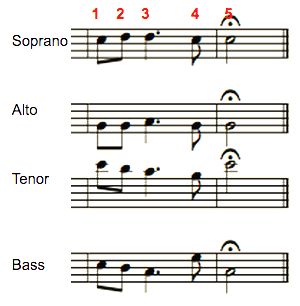
\includegraphics[scale=0.8]{measures}
  \caption{The last 2 measures of a generated composition.}
\end{figure}



\section{Remaining Work}
\subsection{Improvements to evaluation}
In addition to implementing the precision metric as described in the section before, some evaluation of the final product should be implemented, instead of just measuring the models in isolation. There are several ways which this could to be done. First, it may be beneficial to implement a type of theory based metric. The outputted composition could be automatically checked for parallel fifths, dissonant intervals, and other objective measures, and have a score returned based on the number of such mistakes it finds. Additionally, positive elements could be incorporated, where the composition would be checked for contrasting motion, consonant intervals, and either output a separate score or combine it with the negative score. Additionally, some sort of human evaluation could be incorporated, perhaps with experts ranking outputs from different iterations of the algorithm.
\subsection{Improvements to the models}
There are several ways in which our models could be altered or improved in the future. First, the training set could be altered. One interesting way in which the training set could be altered would be to try training on different genres of music, instead of just chorales by Bach. For example, there is no obvious reason why this algorithm would not generalize to other forms of music, including not only classical but even other genres with multiple harmonizing parts, such as barbershop and even pop and rock vocals. Secondly, we could create much more general models by training on a wider array of samples, perhaps from a variety of different genres. This more general model could then be used in conjunction with the more specific models, so that when the context is not found in the more specific model, the algorithm can fall back on the general model.

One other alteration that could be made would be to make a phrase-based translation model, instead of a translation model between single notes. This technique is used frequently in machine translation in order to ensure that the meaning of phrases within a sentence are not lost. For example, instead of translating each word of ``s'il vous pla\^{i}t'' independently, a phrase-based model would translate the whole phrase into the corresponding English phrase ``please''. This idea generalizes well to harmonizing a melody, as there are often sequences of notes that harmonize well into other sequences of notes, which might not be captured by just the single note translation model with the language model. However, this would introduce more sparsity into our data, as there would be more contexts to learn probabilities for, and so a meaningful phrased based model might be difficult to achieve without more data.

In addition to these alterations, more information could be added to each model. A clear example of this would be rhythm information. So far, our algorithm does not take rhythmic variation into account at all. Rhythmic information could be added to the translation model in order to decide what rhythms to generate for the harmony based on the rhythms in the melody. This would probably be fairly difficult to train and decode, as the rhythms have to line up exactly or invalid measures with too many or too few beats may be produced. However, this should still be possible, and would add significantly to the quality of the output if done correctly.
\label{sec:remaining_work}


\bibliographystyle{plain}     % Please do not change the bib-style
\bibliography{progress_report}  % Just the *.BIB filename

\label{app}


\end{document} 

